\chapter{Introducció a la programació en Python}


\section{Terminal de Python}

Al contrari que amb llenguatges com C, C++ o Fortran no necessitem un compilador per a executar el codi en Python. Ser un llenguatge interpretat significa que un programa s'ocupa d'executar el codi Python. El programa que s'encarrega d'aquesta tasca és l'intèrpret. Nosaltres podem interactuar directament amb l'interpret emprant la terminal de Python. Per a obrir-la executem la terminal del sistema i introduïm la comanda {\tt python3} o {\tt python} en el cas de que la versió 3 estigui configurada per defecte al nostre sistema. A la Fig. ~\ref{fig:python-term} es mostra la terminal instal·lada amb Python 3.  Per sortir de la terminal introduirem {\tt exit()} o premerem {\tt Ctrl-D}

\begin{figure}[!h]
    \begin{centering}
    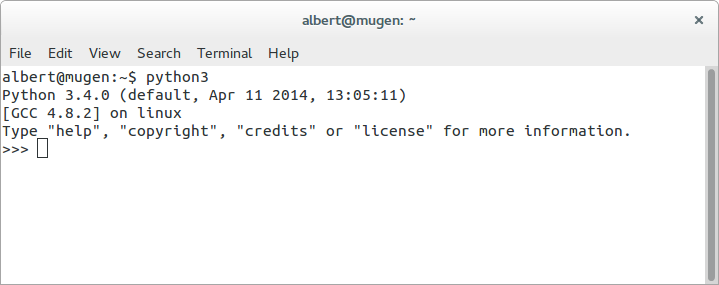
\includegraphics[width=0.8\textwidth]{img/python-term.png}
    \caption{Terminal de Python 3}
    \label{fig:python-term}
    \end{centering}
\end{figure}


\subsection{Primer programa en Python}


A informàtica el primer programa que s'implementa s'anomena \emph{Hello world}. Consisteix en mostrar per la terminal aquesta cadena de caràcters. Per a executar aquest exemple obrim un intèrpret de Python i hi introduïm el següent codi.



\begin{tip}[caption=Hello world]
>>> print("Hello world")
Hello world
\end{tip}




Veurem que el resultat és la cadena de caràcters passada com a paràmetre a la funció. En aquest exemple s'ha cridat la funció {\tt print()} que imprimeix per pantalla cadenes de caràcters passades com a paràmetre. Si provem amb altres arguments veurem com sempre rebrem com a sortida la cadena de caràcters introduïda. 


Com hem comentat abans Python es troba en una transició entre la versió 2 i 3, tot i que la versió 3 és completament funcional. Podem obrir un intèrpret de Python 2 executant la comanda {\tt python2} o {\tt python} (si la versió 2 es troba configurada per defecte) i introduïm el següent exemple de {\tt Hello world} sense parèntesis. 


\begin{blockcode}
>>> print "Hello world"
Hello world
\end{blockcode}

Ara provem a executar aquest mateix exemple amb Python 3 i comprovem els resultats. En Python 3 la funció {\tt print} ha passat a ser considerada una funció més i els paràmetres han de ser cridats sempre entre parèntesis.


\section{Terminal iPython}


El software iPython és una terminal de Python enriquida. Té diversos mòduls implementats com la consola basada en la llibreria gràfica Qt, el quadern de codi iPython Notebook, suport per a la visualització integrada de gràfics a la terminal o eines per facilitar el còmput d'altes prestacions. No es troba instal·lada per defecte, així que s'haurà d'afegir al software del nostre sistema. Per a executar-la haurem de cridar la comanda {\tt ipython} o {\tt ipython3}. Té una llarga llista de funcionalitats i podem executar algunes comandes del sistema des iPython. Per veure una referència breu intruir {\tt \%quickref}, i per a sortir d'aquest premerem la tecla \emph{Q}. A la Fig. ~\ref{fig:ipython-term} es mostra la terminal iPython en funcionament.

\begin{figure}[!h]
    \begin{centering}
    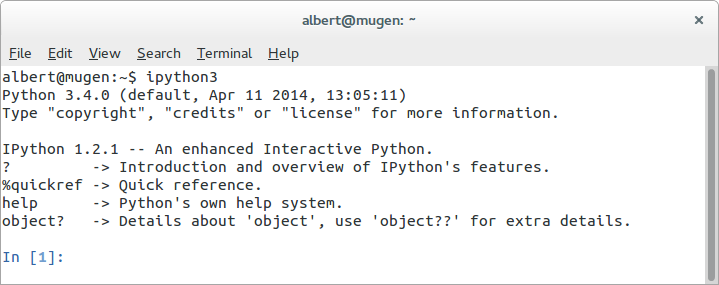
\includegraphics[width=0.9\textwidth]{img/ipython-term.png}
    \caption{Terminal de iPython}
    \label{fig:ipython-term}
    \end{centering}
\end{figure}


Un dels avantatges més productius de la terminal és l'autocompletat. Aquesta funcionalitat ens mostrarà totes les opcions que tenim donada un conjunt de lletres, un objecte, un mòdul, etc. Per a provar-ho introduir la lletra \emph{p} i prémer la tecla \emph{Tab}. Es veurà el conjunt de comandes que comencen amb la lletra \emph{p}.



\begin{blockcode}
>>> p
%%perl      %%python    %paste      %pdef       %pinfo      
%pprint     %prun       %pushd      %pylab      pow         
%%prun      %%python3   %pastebin   %pdoc       %pinfo2     
%precision  %psearch    %pwd        pass        print       
%%pypy      %page       %pdb        %pfile      %popd       
%profile    %psource    %pycat      plt         property
\end{blockcode}




IPython permet guardar en un arxiu totes les comandes introduïdes durant una sessió. Per a desar-les s'ha de cridar a la funció {\tt save} amb el següent format: {\tt \%save nom\_sessió id\_comandes}. A iPython cada comanda té un identificador numèric. Per a introduir rangs de comandes es separen per guió i per comandes individuals s'introdueixen soles com a l'exemple següent.

\begin{blockcode}
>>> %save sessio_avui 3-10 15-20 22 28
\end{blockcode}



Podem consultar les propietats d'un objecte en Python que pot ser una funció, mòdul, variable, etc. Per a fer-ho introduïm el nom del objecte seguit del símbol d'interrogació. Per exemple consultem les propietats de la funció {\tt print()}.

\begin{blockcode}
>>> print?
Type:       builtin_function_or_method
String Form:<built-in function print>
Namespace:  Python builtin
Docstring:
print(value, ..., sep=' ', end='\n', file=sys.stdout, 
flush=False)

Prints the values to a stream, or to sys.stdout by default.
Optional keyword arguments:
file:  a file-like object (stream); defaults to the current 
sys.stdout.
sep:   string inserted between values, default a space.
end:   string appended after the last value, default a newline.
flush: whether to forcibly flush the stream.
\end{blockcode}

Quan estiguem treballant amb iPython i estem modificant el nostre codi font les llibreries importades no es modificaran per defecte i haurem de tancar la terminal i torar a entrar. Per evitar-ho activem l'opció {\tt autoreload} de iPython amb les següents comandes.


\begin{blockcode}
>>> %load_ext autoreload
>>> %autoreload 2
\end{blockcode}


\section{Executant el nostre codi Python}

La terminal és còmode per a realitzar probes i molt útil per a l'aprenentatge, però per a projectes ens interessarà crear el nostre propi programa en un fitxer. Per a desar el nostre codi creem un arxiu anomenat {\tt programa.py} i hi introduïm el següent codi.

\begin{blockcode}
#!/usr/bin/env python3
print("Hello world")
\end{blockcode}


La directiva {\tt \#!/usr/bin/env python3} s'ocupa de buscar on és l'intèrpret de Python 3 d'una manera portable entre plataformes Unix. Un cop tenim el nostre codi Python hi han dues maneres d'executar-lo. Una és passar-li la ruta al fitxer com a paràmetre a l'intèrpret de Python. Suposant que hem desat el fitxer a la nostra carpeta d'inici.


\begin{blockcode}
$ python3 programa.py
Hello world
\end{blockcode}

Una altra manera és donar-li permisos d'execució al nostre programa. Per a això hem d'utilitzar la comanda {\tt chomd} de Unix i amb el paràmetre {\tt +x} que afegeix permisos d'execució a un fitxer. Un cop tenim permisos podem executar el binari especificant-li la ruta {\tt ./} més el nom {\tt programa.py}.

\begin{blockcode}
chmod +x programa.py
./programa.py
Hello world
\end{blockcode}

Un tercera manera és executar el programa des de la terminal. Per això hem de cridar a la funció {\tt run} i especificar-li la ruta del programa i el nom.
  
\begin{blockcode}
>>> run "programa.py"
Hello world
\end{blockcode}

\subsubsection*{Exercici \Roman{exercici}} \stepcounter{exercici}


Executar l'exemple anterior amb la terminal iPython, guardar--lo i executar-lo des de la terminal.


\subsubsection*{Exercici \Roman{exercici}} \stepcounter{exercici}


Executar l'exemple anterior amb la terminal iPython, desar-lo en una carpeta anomenada {\tt exemple} i executar-lo des de la terminal. Com accedeixes a la ruta del arxiu?



\section{Paraules reservades}


Hi ha un conjunt de paraules que son reservades del llenguatge i no es poden emprar per a anomenar mòduls, llibreries, variables, funcions, etc. Si ho provem ens donarà un error.

{\tt and assert break class continue def del elif else except \\
exec finally for from global if import in is lambda not or pass \\
print raise return try while yield}




  
\section{Comentaris de codi}



Els comentaris de codi permeten introduir text en el programa sense que sigui interpretat. Ens permet introduir descripcions als nostres programes i descriure'ls per a que qualsevol que el llegeixi entengui què fa el sistema. També s'utilitza per a fer que part del codi no s'executi. Hi han dos menes de comentaris.


\begin{itemize}
    \item Comentaris de línia: emprem \#
    \item Comentaris de bloc: emprem cometes triples $""" comentari """$
\end{itemize}

\begin{blockcode}
#!/usr/bin/env python3
# -*- coding: utf-8 -*-

"""
Autor: Albert Gutiérrez Millà
Data: 25 de juny del 2014
"""

# Aquesta funció retorna la cadena de caràcters per la stdout
print("Hello world")
\end{blockcode}


